This sping-mass-pendulum-based example is presented to introduce \textit{bioptim}'s ability to use of external forces.
The goal was to maintain the position of a $\SI{1}{kg}$ mass hanging on a linear spring attached to the ground.
A $\SI{0.2}{m}$-long pendulum weighting $\SI{10}{kg}$ was attached to the mass and free to rotate in one dimension (Fig.~\ref{fig:Mass_Pendulum_Model}).
In addition to the spring force, the mass was actuated by a vertical force (e.g., somebody pulling on it) while the pendulum rotation was passive.
The system therefore comprised two DoFs, the mass position ($q_m$) and the pendulum angle ($q_p$) and one control input, the vertical force pulling on the mass ($f$). 
\begin{figure}[h!]
\centering
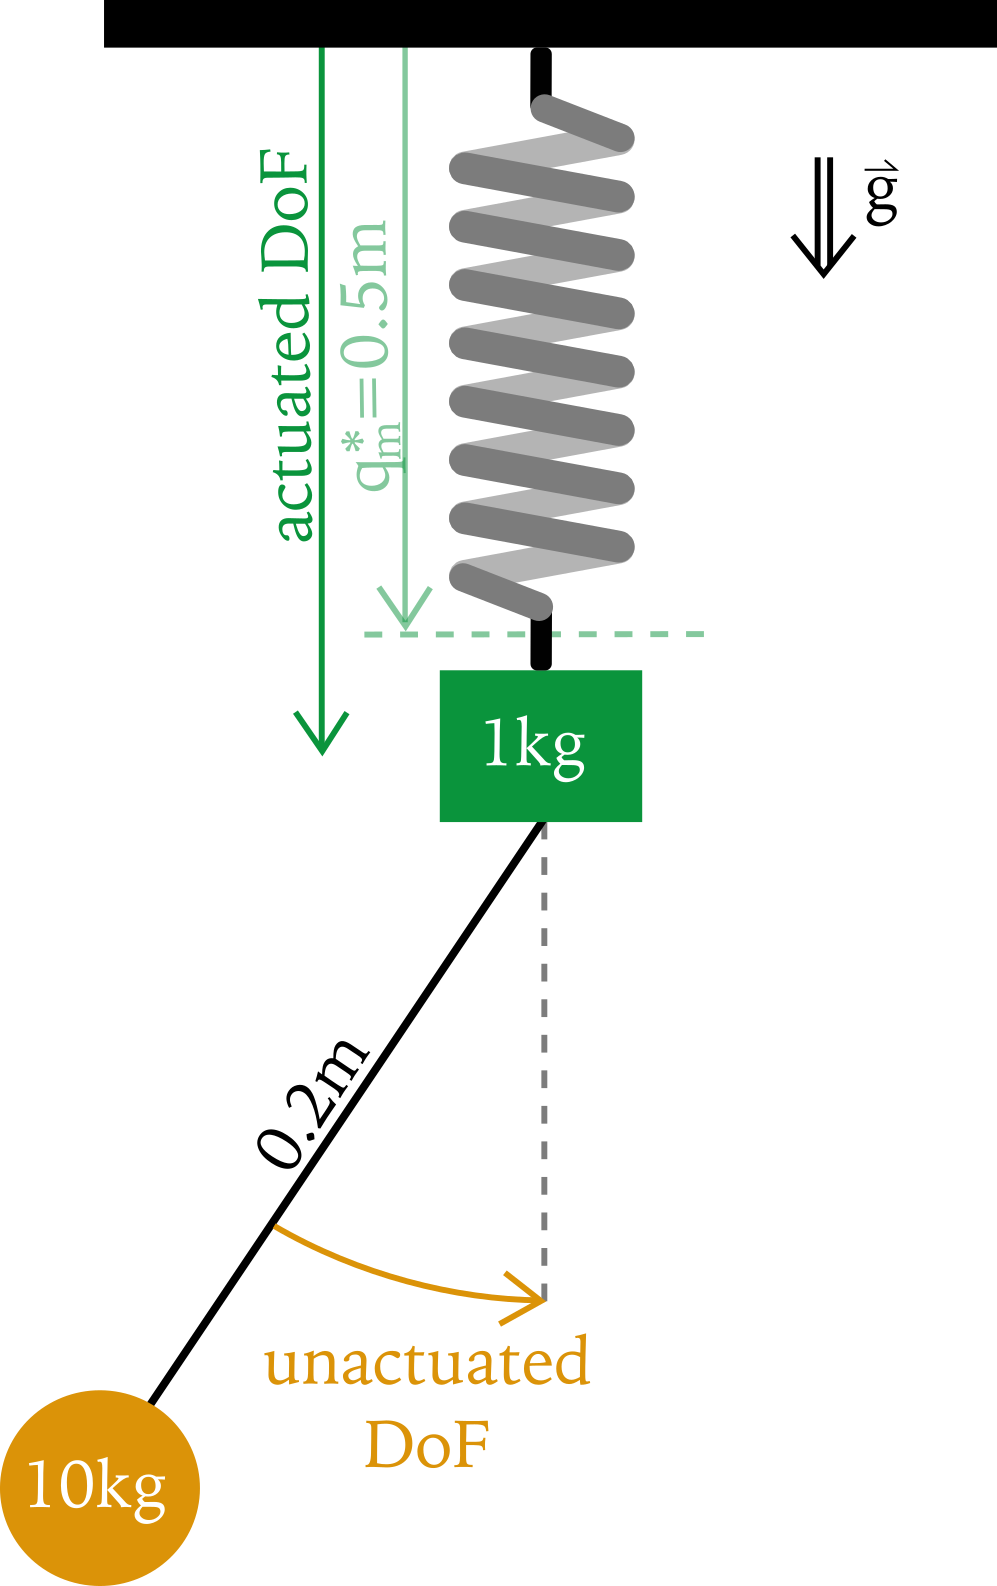
\includegraphics[width=0.35\columnwidth]{figures/Mass_Pendulum_Model.png}
\caption{Definition of the spring-mass-pendulum model.}
\label{fig:Mass_Pendulum_Model}
\end{figure}
The spring force was:
\[
\begin{aligned}
F_{ext} = -k*q_m,
\end{aligned}
\addtag
\label{eq:f_ext}
\]
with k the spring stiffness constant.\\
The objective function, composed of Lagrange terms, was formulated as follow:
\[
\mathcal{J} = \underbrace{\int_{T/2}^T (q_m + 0.5)^2~dt}_{\mathtt{TRACK\_STATE}}  +~\omega_1 \underbrace{\int_{T/2}^T ~\tau^2~dt}_{\mathtt{MIN\_ TORQUE}},
\addtag
\label{eq:ocp_Pendulum}
\]

\noindent with $q_m$ the position of the mass, $\omega_1 = 1\times 10^{-6}$, T the duration of the movement and $\tau$ the force control of the mass.
The first term of the objective function (Eq.~\ref{eq:ocp_Pendulum}) acts as a position controller for the mass.
\comment{The second and third}{je n'en vois qu'un} were added for control regularization.

The OCP was composed of two phases each lasting for $\SI{5}{s}$, with 50 shooting nodes.
In the first phase, no objective function was minimized and $f$ was constrained to $0$ letting the mass oscillating freely. 
Then, in the second phase, $\mathcal{J}$ was minimized, stabilizing the mass around the targeted position (Fig.~\ref{fig:Mass_Pendulum_Fext_graphs}).
This example highlights the possibility of using optimal control to find activation patterns compensating for external passive forces (e.g., \comment{ortheses flexibility, }{trouver d'autre}).

\begin{figure*}[t!]
\centering
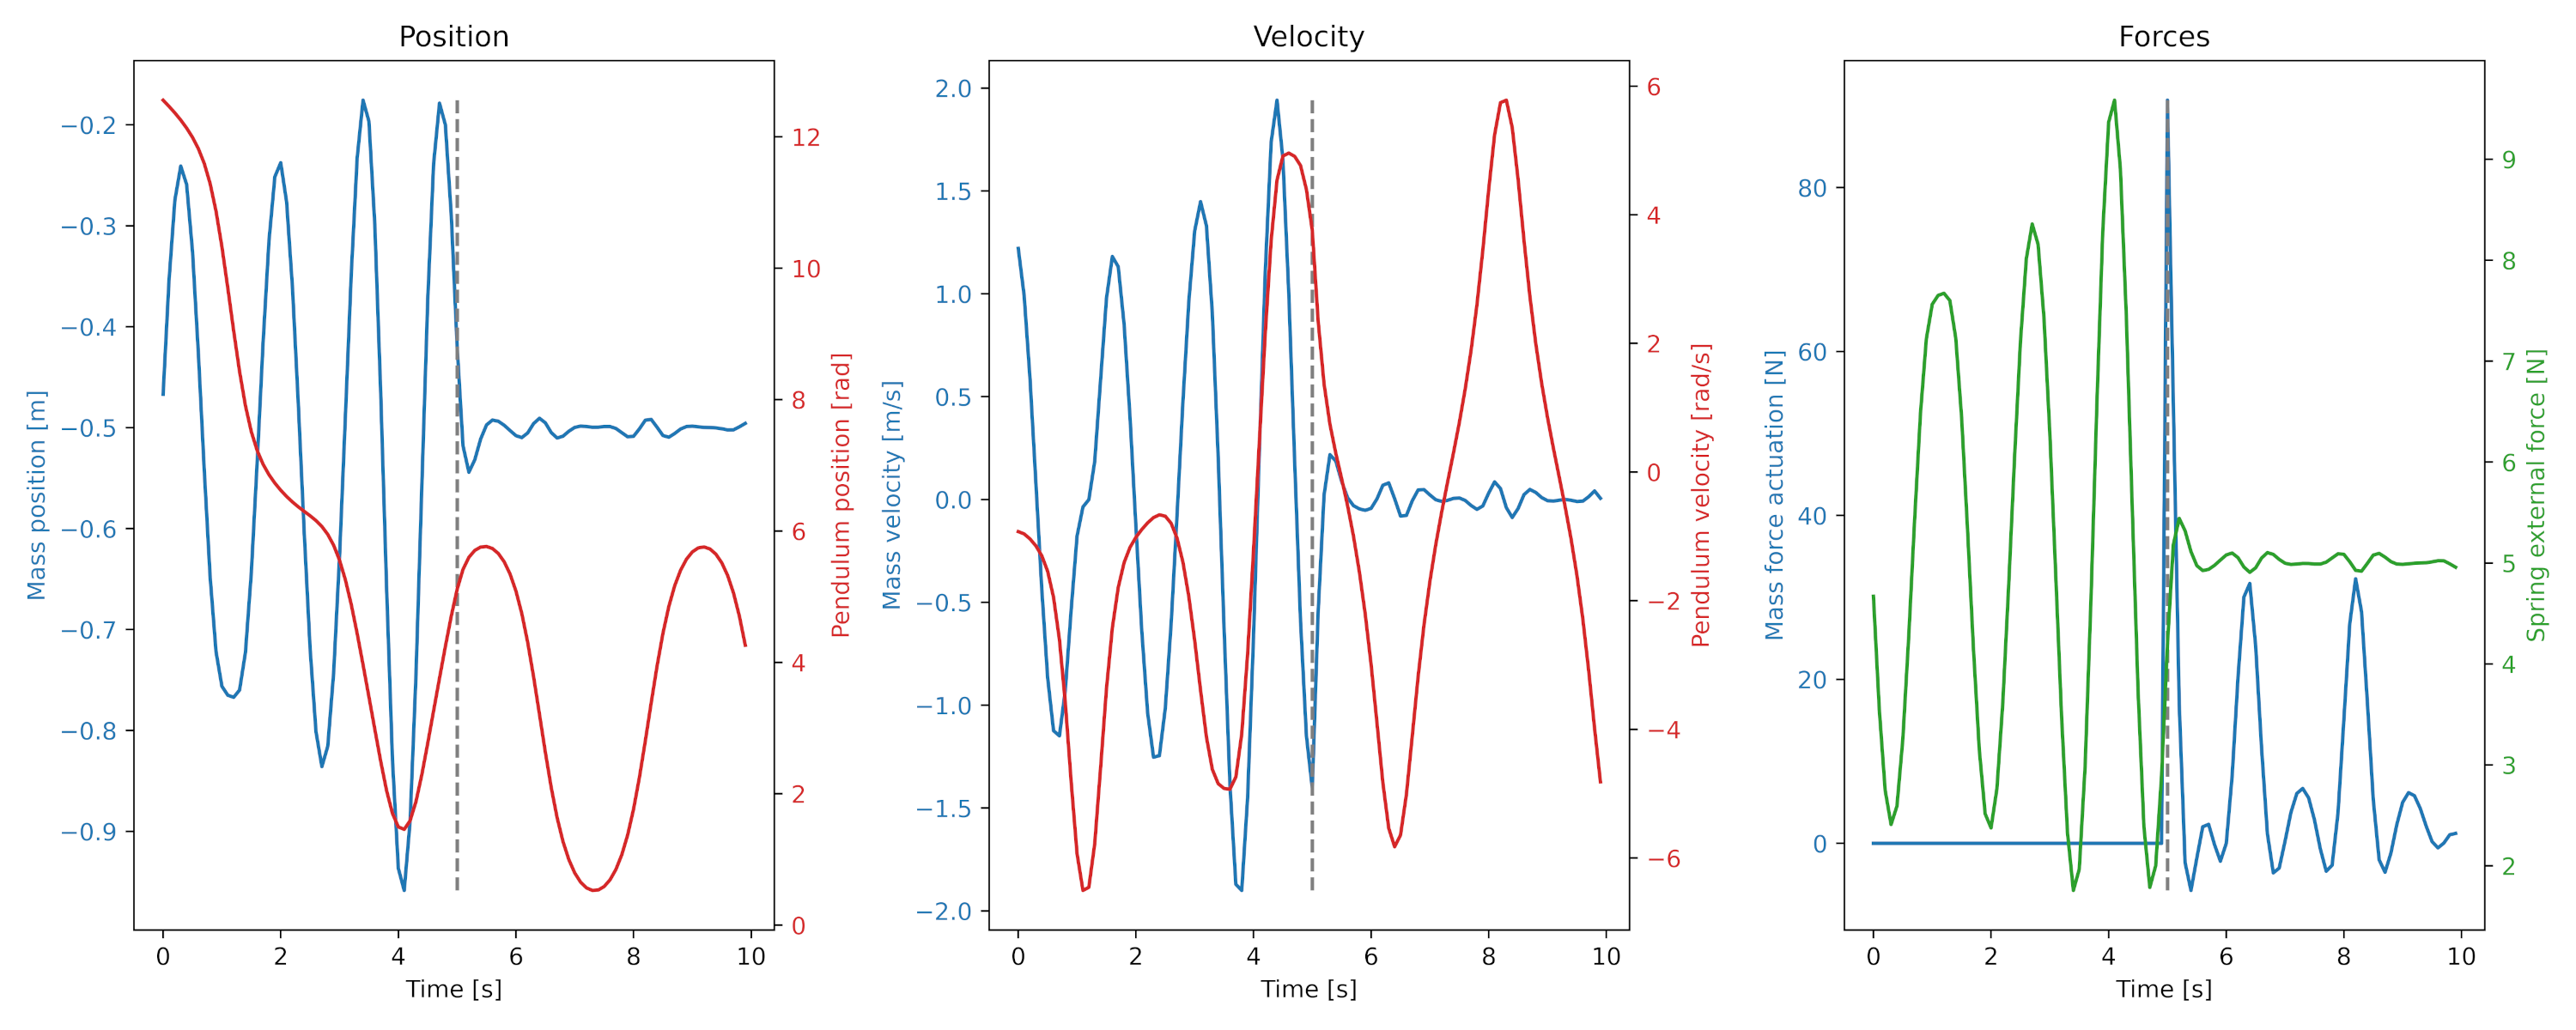
\includegraphics[width=\textwidth]{figures/Mass_Pendulum_Fext.png}
\caption{Optimal kinematics of the mass-pendulum-spring system. Gray dashed lines show the stage transition, blue lines are related to the mass, red lines are related to the pendulum and the green line is related to the spring.}
\label{fig:Mass_Pendulum_Fext_graphs}
\end{figure*}














